\subsubsection{Visual and Statistical Analysis of \ce{SiO_2} Distribution in Partitioned Data}\label{sec:visual_analysis}
This section presents a detailed visualization and statistical analysis of \ce{SiO_2} concentration distribution across different folds, which are the result of our data partitioning procedure on the dataset we use.
The analysis focuses on \ce{SiO_2} as a representative example, with similar analyses conducted for other oxides but omitted here for brevity.

Figures \ref{fig:histogram_grid_plot} and \ref{fig:histogram_kde_plot} illustrate the histograms and \gls{kde} curves for \ce{SiO_2} concentrations in each training fold, the test set, and their combined distributions.
The consistent histograms and \gls{kde} curves across different training folds indicate that the data distribution within each fold closely matches the overall distribution.
The high degree of overlap among the combined distributions across training folds and the test set further confirms their consistency and representativeness.

Figure \ref{fig:original_and_post_fold_plot} contrasts the \ce{SiO_2} concentration distribution before and after data partitioning.
The left plot shows the original distribution, while the right plot displays the fold-assigned distribution, color-coded by fold.
This visualization highlights that the partitioning strategy maintains the overall data distribution while ensuring balanced representation across folds.

These visual analyses collectively validate our k-fold data partitioning method.
They demonstrate that each fold provides a reliable estimate of model performance and help prevent overfitting by training and validating on similarly distributed data.

\begin{figure*}[h!]
    \centering
    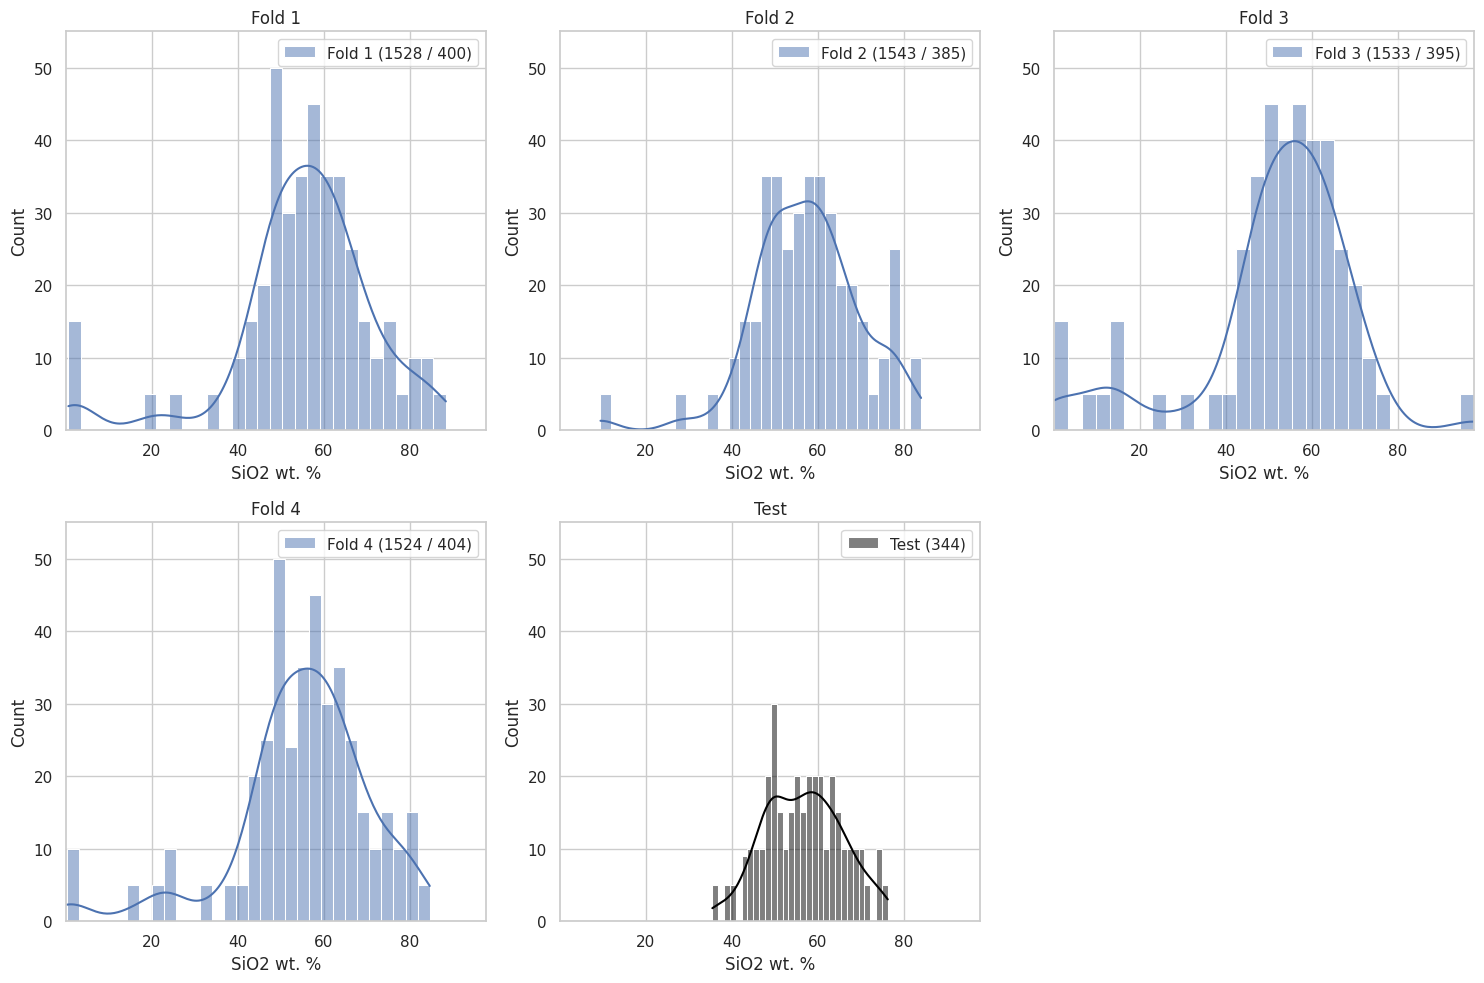
\includegraphics[width=\textwidth]{images/histogram_grid_plot.png}
    \caption{Histogram and \gls{kde} of \ce{SiO_2} Distribution in Each Fold. The y-axis represents the count of samples per bin, and the x-axis represents \ce{SiO_2} concentration. The notation in the legend indicates the amount of instances in the training/validation sets.}
    \label{fig:histogram_grid_plot}
\end{figure*}

\begin{figure*}[h!]
    \centering
    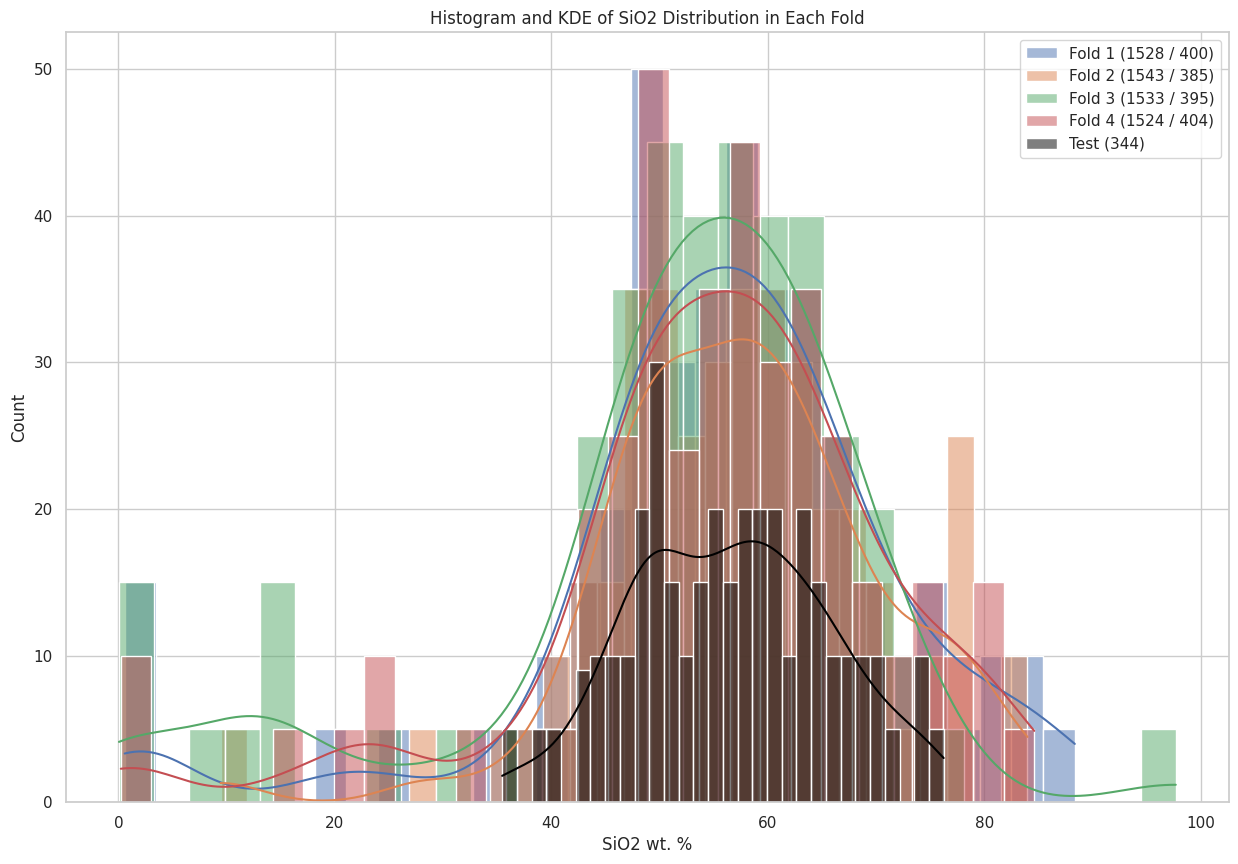
\includegraphics[width=\textwidth]{images/histogram_kde_plot.png}
    \caption{Combined Histogram and \gls{kde} of \ce{SiO_2} Distribution in Each Fold. The y-axis represents the count of samples per bin, and the x-axis represents \ce{SiO_2} concentration. The notation in the legend indicates the amount of instances in the training/validation sets.}
    \label{fig:histogram_kde_plot}
\end{figure*}

\begin{figure*}[h!]
    \centering
    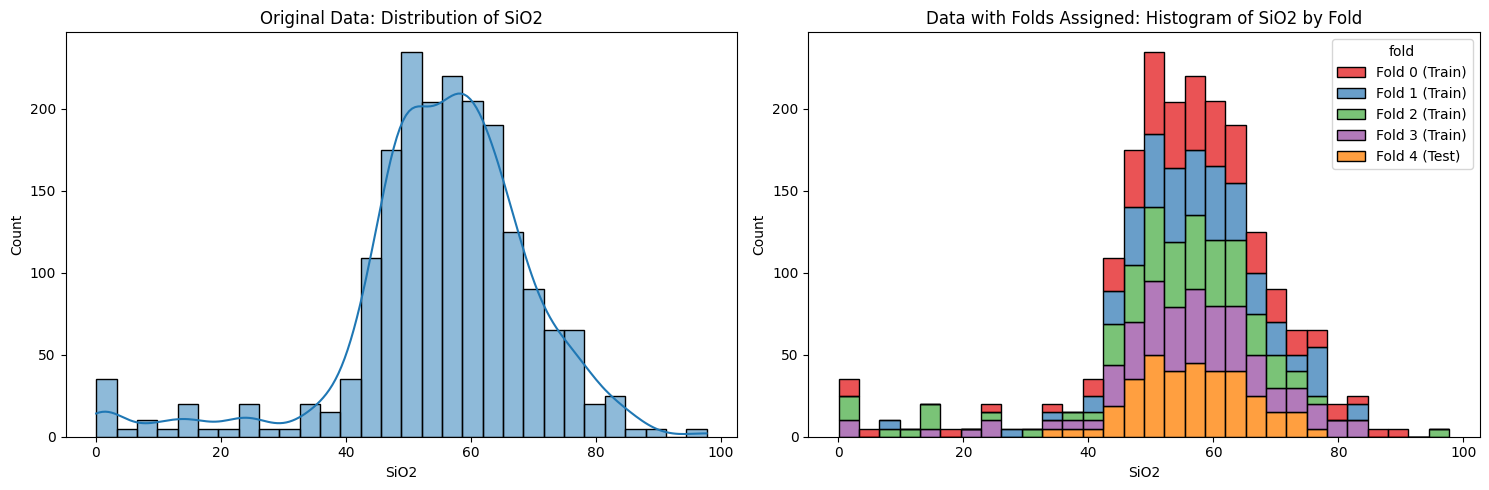
\includegraphics[width=\textwidth]{images/original_and_post_fold.png}
    \caption{Distribution of \ce{SiO_2} concentrations before and after fold assignment. The left plot shows the original distribution of \ce{SiO_2}, while the right plot shows the distribution with folds assigned, color-coded to indicate the different folds.}
    \label{fig:original_and_post_fold_plot}
\end{figure*}


To further validate our visual analysis, we can look at quantitative measures such as the means and standard deviations of \ce{SiO_2} concentrations across the folds and the overall dataset.

\begin{figure*}[htbp]
    \centering
    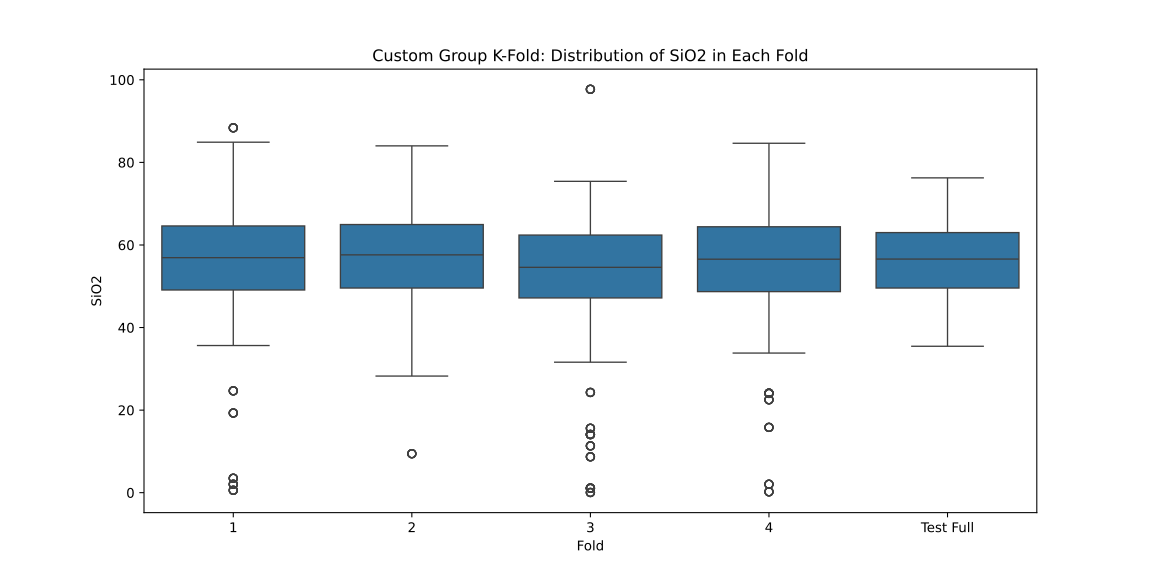
\includegraphics[width=\textwidth]{images/distribution_plot.png}
    \caption{Distribution of \ce{SiO_2} concentrations across cross-validation folds, training set, test set, and the entire dataset. The mean and standard deviation statistics for each partition are indicated figure.}
    \label{fig:siO2_distribution}
\end{figure*}

From Figure~\ref{fig:siO2_distribution}, it is evident that the means and standard deviations of \ce{SiO_2} concentrations for each fold, as well as the combined training set, are consistent with those of the full dataset.
This quantitative consistency supports the visual evidence that each training fold is representative of the entire dataset.
Furthermore, we can see that the standard deviation in the training sets is higher than the standard deviation in the test set, which is expected given the reassignment of extreme values to the training sets.

Maintaining balanced and representative distributions in each fold is essential for training robust models.
It ensures that the models are not biased towards any specific subset of the data, which is crucial for their generalization to unseen data.
The balanced distributions across folds enable the model to be trained on diverse subsets of data, leading to better generalization.
This approach reduces the risk of overfitting and ensures that the model performs well on new, unseen data.

By ensuring that each fold is representative of the overall dataset, these visualizations support the validity of our dataset partitioning strategy.
The consistency observed across folds further supports the claim that the data distribution method works as intended, providing confidence in the generalizability and reliability of our models.